\chapter{The \lhcb detector}
\label{sec:detector}

Most parts of this chapter are taken from \cite{detector}

The \lhcb experiment is one of the four big experiments, currently running at the Large Hadron Collider (LHC) of the European Organization for Nuclear Research CERN in Geneva, Switzerland. In contrast to the other three experiments -- \atlas and \cms are searching for direct hints of new physics, \alice investigates the Quark-Gluon-Plasma -- \lhcb is dedicated to look indirectly for physics beyond the Standard Model (see section \ref{sec:Theory}) by the study of hadrons containing either a heavy \bquark- or \cquark-quark.

...

The layout of the \lhcb detector can be seen in figure \ref{fig:detector}. It is built as a single-arm forward spectrometer. The reason for this choice is, that at \lhc energies of $\sqs = 14 \tev$ at the maximum, \bquark- and \bquarkbar- hadrons are predominantly produced in the forward (or backward) region.

\begin{figure}[hptb]
	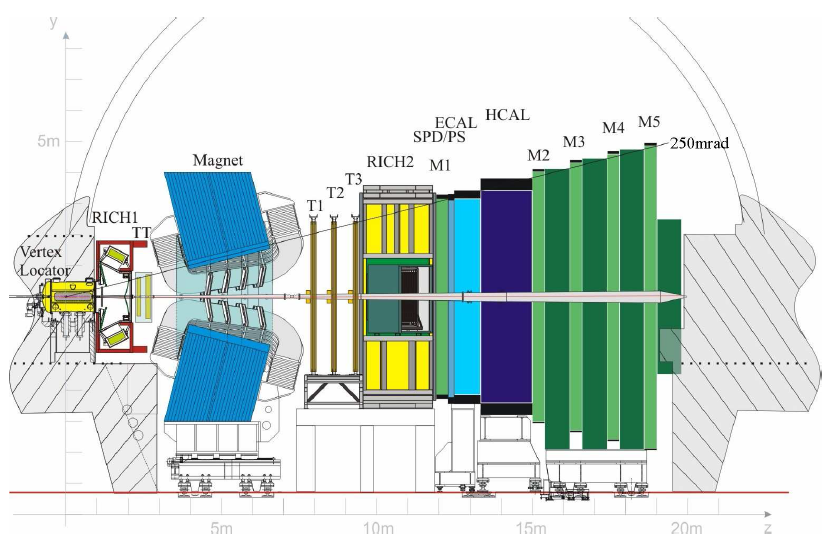
\includegraphics[width=\textwidth]{lhcb-detector}	
	\caption{The \lhcb detector.}
	\label{fig:detector}
\end{figure}

% ===========================
% SECTION: Tracking detectors
% ===========================
\section{Tracking detectors}
Tracking describes the whole procedure to reconstruct the trajectories of the (charged) particles produced in the proton-proton collision. If there's a magnet in use, the particles' charges and momenta can be determined as well. For that purpose, a system of several subdetectors is aligned up- and downstream the dipole magnet, namely the Vertex locator (VELO), the Trigger Tracker (TT) and the Trigger stations (T1-T3) built-up by the Inner Tracker (IT) and the Outer Tracker (OT).

\subsection{Vertex locator (VELO)}

\subsection{Trigger Tracker / Tracker Turicensis (TT)}

\subsection{Inner Tracker (IT)}

\subsection{Outer Tracker (OT)}

\subsection{Track classification}


% ================================
% SECTION: Particle identification
% ================================
\section{Particle identification}

\subsection{Ring Imaging Cherenkoy Detector (RICH)}

\subsection{Calorimeter system}

\subsection{Muon chambers}

% ===========================
% SECTION: Trigger
% ===========================
\section{Trigger}

\subsection{L0-Trigger}

\subsection{High Level Trigger (HLT)}